\begin{IEEEbiography}[{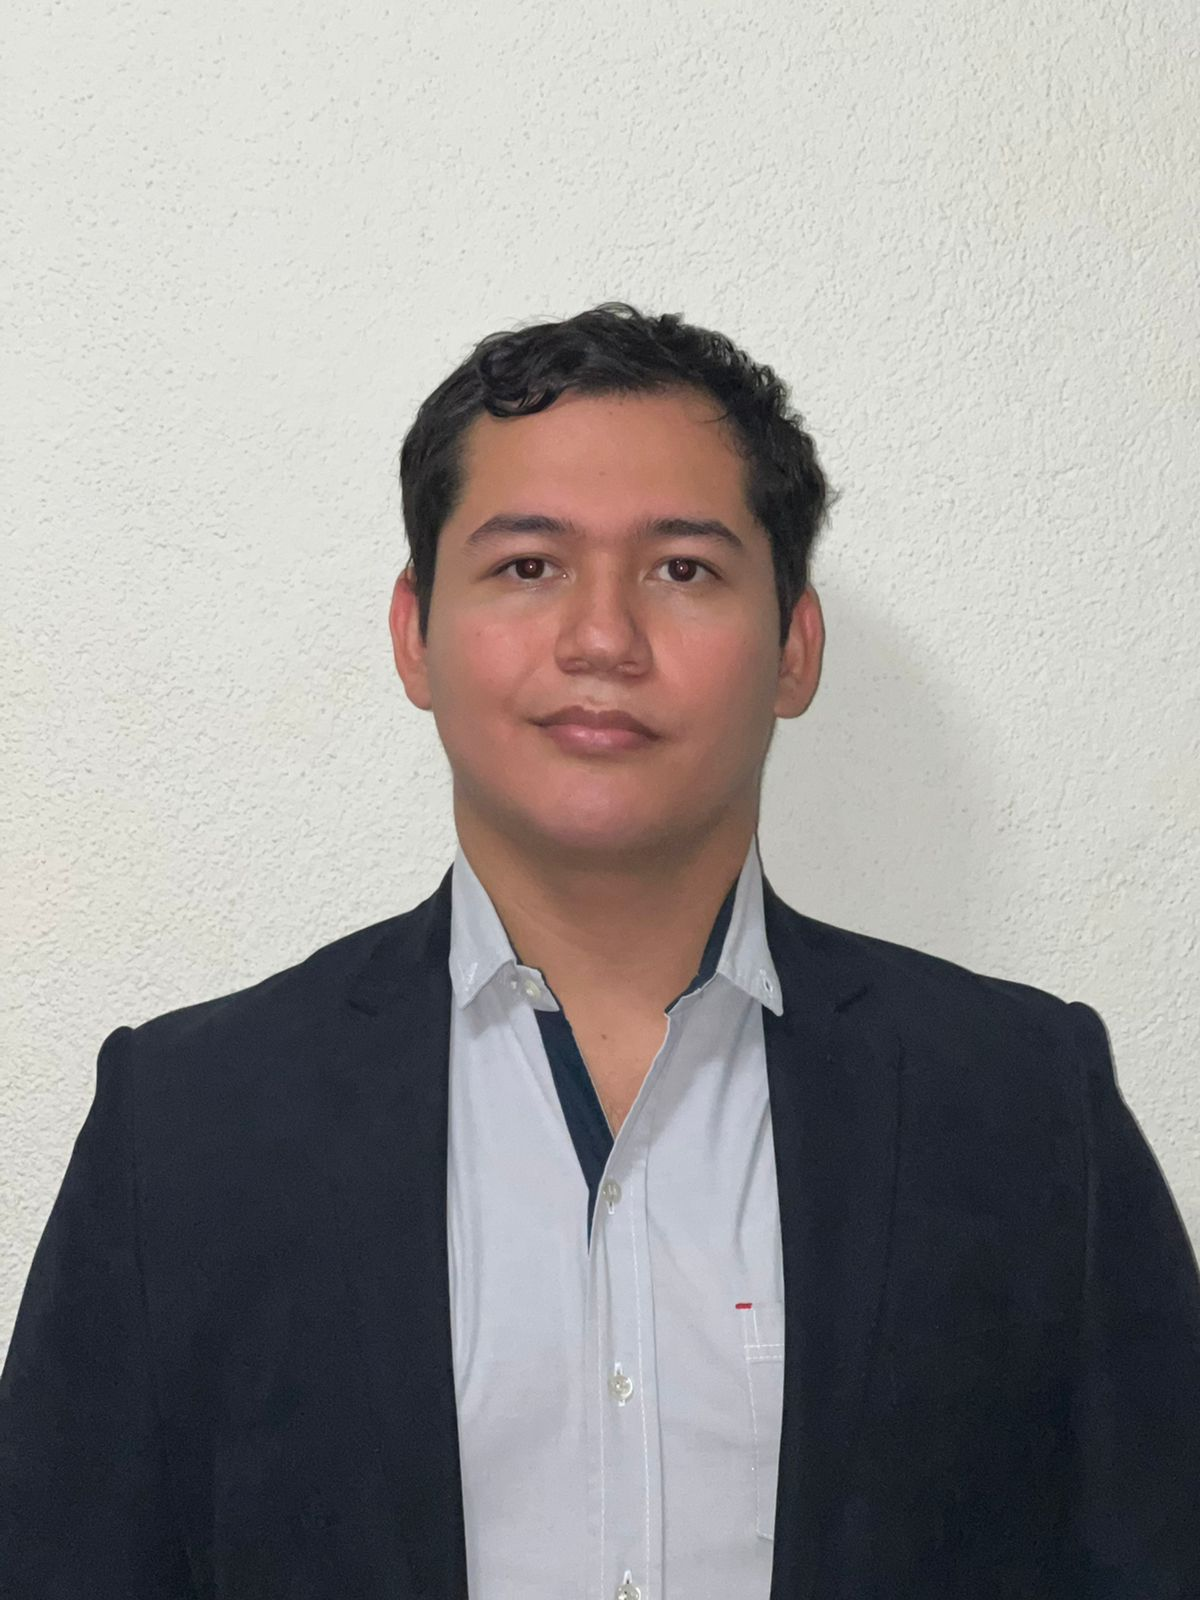
\includegraphics[width=1in,height=1.25in,clip,keepaspectratio]{Pictures/angel.jpg}}]{Angel Orellana}
Angel Orellana is a student of electronic engineering at Universidad del Valle 
de Guatemala. He has a passion for designing analog and digital circuits, 
programming, and telecommunications.
\end{IEEEbiography}
    
\begin{IEEEbiography}[{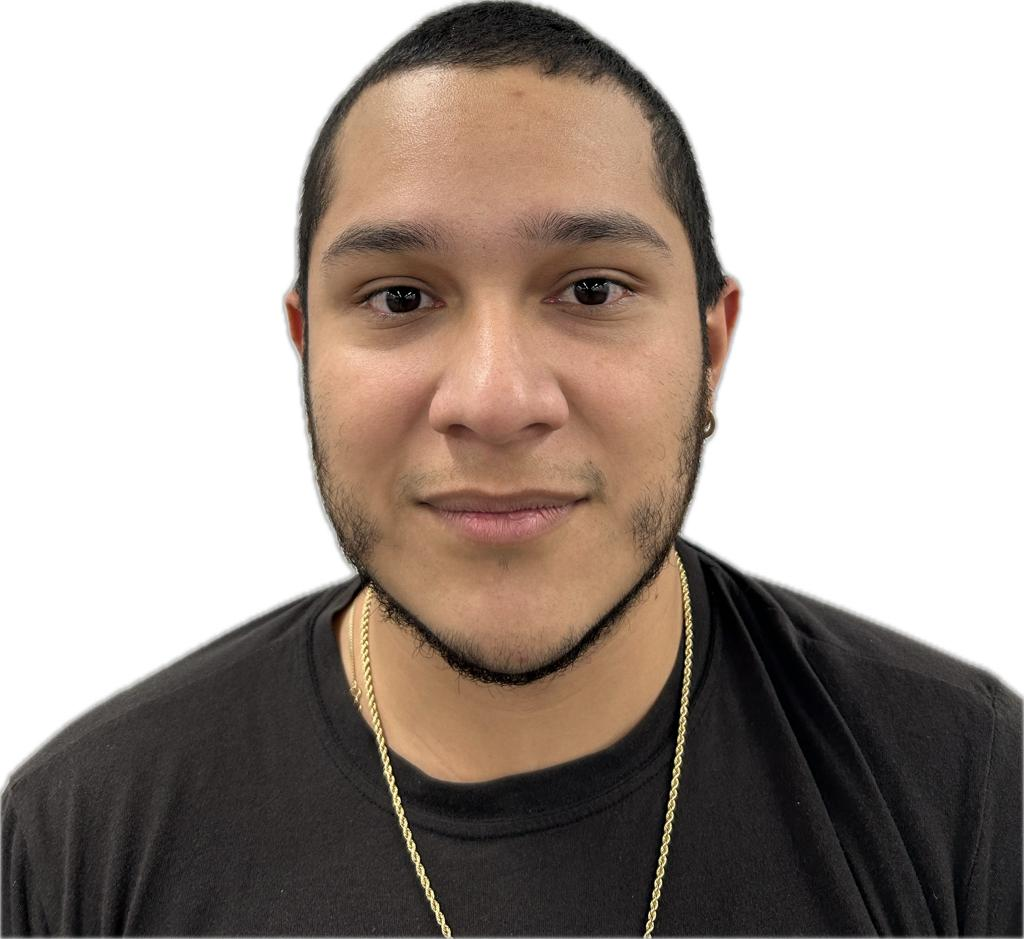
\includegraphics[width=1in,height=1.25in,clip,keepaspectratio]{Pictures/Julio.jpg}}]{Julio E. Lopez}
was born in Guatemala city in 1999 April 20th. Lived in San Ignacio, Cayo Belize. Went to school at
St. Andrews Primary school then, moved forward to Sacred heart High school to do 2 of
his 4 years of high school then he moved out of his house to live on his own for the last
two years of high school at the great and prestige St. Johns college where when graduated from
arts and physics majors. Through all of his schooling he was a player in the St. Andrews, Sacred Heart school , And St Johns
college basketball, and the starter of 3 clubs at St Johns college, the anime club the travel club, and lastly, the
rescue and support club which started base on the hurricane that hit Belize in 2018.
\end{IEEEbiography}